\documentclass[journal]{IEEEtran}

%\usepackage[brazil]{babel}
%\usepackage[T1]{fontenc}

\usepackage{theorem}        %%Lo agregue yo <========================================
\usepackage{algorithmic}        %%Lo agregue yo <========================================

\setcounter{secnumdepth}{7}

\newtheorem{theorem}{Theorem}%[section]
%\newtheorem{acknowledgement}[theorem]{Acknowledgement}
%\newtheorem{algorithm}[theorem]{Algorithm}
%\newtheorem{axiom}[theorem]{Axiom}
%\newtheorem{case}[theorem]{Case}
%\newtheorem{claim}[theorem]{Claim}
%\newtheorem{conclusion}[theorem]{Conclusion}
%\newtheorem{condition}[theorem]{Condition}
%\newtheorem{conjecture}[theorem]{Conjecture}
%\newtheorem{criterion}[theorem]{Criterion}
%\newtheorem{exercise}[theorem]{Exercise}
%\newtheorem{notation}[theorem]{Notation}
%\newtheorem{problem}[theorem]{Problem}
%\newtheorem{proposition}[theorem]{Proposition}
\newtheorem{remark}[theorem]{Remark}
%\newtheorem{solution}[theorem]{Solution}
%\newtheorem{summary}[theorem]{Summary}

\newtheorem{definition}[theorem]{Definition}
\newtheorem{example}[theorem]{Example}
\newtheorem{lemma}[theorem]{Lemma}
\newenvironment{proof}[1][Proof]{\textbf{#1.} }{\ \rule{0.5em}{0.5em}}
\newtheorem{corollary}[theorem]{Corollary}
\newenvironment{algorithm}[1][Algorithm]{\textbf{#1.} }{}

\usepackage{amssymb}
\usepackage{graphicx}
\usepackage{amsmath}
\usepackage{psfrag}

\usepackage{accents}
%\usepackage[none]{hyphenat}

\usepackage[usenames,dvipsnames,svgnames,table]{xcolor}

\hyphenation{bet-ween re-pre-sen-ting} %
\sloppy

\begin{document}

\title{New Results of Optimal Rate in Joint Source-Channel Coding of Correlated Sources}


\author{---------- ---------- ---------- ---------- ---------- %%%%Fernando P. Rivera and Jaime Portugheis
\thanks{Manuscript received XXXX XX, 2014; revised XXXXX XX, 2014.}
\thanks{---------- ---------- ---------- ---------- ---------- ---------- ---------- ---------- ---------- ---------- ---------- }%%%%Fernando P. Rivera is with Department of Communications, State University of Campinas, Campinas, SP, Brazil. Email:fpujaico@decom.fee.unicamp.br. }
\thanks{---------- ---------- ---------- ---------- ---------- ---------- ---------- ---------- ---------- ---------- ---------- }}%%%%Jaime Portugheis   is with Faculty of Technology       , State University of Campinas, Limeira , SP, Brazil. Email:jaime@ft.unicamp.br  .}}

\markboth{IEEE Communications Letters,~Vol.~X,
No.~XX,~XXXXX~XXX}{Shell \MakeLowercase{\textit{et al.}}: Bare
Demo of IEEEtran.cls for Journals}

% make the title area
\maketitle
%%%%%%%\IEEEpeerreviewmaketitle


\begin{abstract}
This paper proposes a method to improve the computational cost of the calculus the optimal rate in 
joint source-channel coding of a set of correlated sources. Here is analyzed 
the case when the sources  are so far of the joint decoder, so that the channel 
capacities  are approximately same. We got lower the complexity of calculus of 
the optimal rate, for $M$ correlated sources, so that the complexity grows linearly 
with $M$.

\end{abstract}

\begin{keywords}
Multiple correlated sources, large scale sensor networks, source-channel coding.
\end{keywords}

\IEEEpeerreviewmaketitle
%%%%%%%%%%%%%%%%%%%%%%%%%%%%%%%%%%%%%%%%%%%%%%%%%%%%%%%%%%%%%%%%%%%%%%%%%%%%%%%%%%%%%%%
%%%%%%%%%%%%%%%%%%%%%%%%%%%%%%%%%%%%%%%%%%%%%%%%%%%%%%%%%%%%%%%%%%%%%%%%%%%%%%%%%%%%%%%
%%%%%%%%%%%%%%%%%%%%%%%%%%%%%%%%%%%%%%%%%%%%%%%%%%%%%%%%%%%%%%%%%%%%%%%%%%%%%%%%%%%%%%%
\section{Introduction}
\label{sec:Intro}

 In the work seen in \cite{fernando}, they are presented equations to the calculus of two cases the 
 optimal minimum rates in joint source-channel coding of a set of correlated sources;
 thus, were showed methods for to get the minimal,  common rate and  sum rate.
 These  rates fulfill the Slepian-Wolf 
 \cite{slepian} and channel capacity limit \cite{cover} theorems.
 %This sources transmit your codified information across $M$ orthogonal
 %channels to a joint decoder. 
 The results show that, the calculus of 
 the optimal rates of $M$ correlated sources grows in complexity exponentially 
 with $M$.  
 
 In this paper, is assumed the same system 
 model and analyzed the same two cases presented 
 in \cite{fernando}, with the additional restriction that the 
 sources are so far of the joint decoder, in comparing with the distance 
 between sensors, so that the channel capacities in all channels are 
 approximately same. By other side, the correlation values between sources are
 assumed as random or with spatial correlation \cite{corrspatial},
 in contrast with studied in \cite{ceobinary1,ceobinary2}, where the correlation values
 between any source pair is same. 
 
 Other restriction, considered in this article it is the use of a specific model 
 of correlated sources; being used a model similar to seen
 in \cite{ceobinary1,ceobinary2}; where $M$
 correlated sources are generates passing a common source across $M$ binary 
 symmetric channels ($BSC$).
 Using all these considerations, it can be deduced for the calculus of optimal common rate, a method 
 with a calculus complexity that grows linearly with the number of sources, 
 and for the calculus of optimal sum rate a method with \textcolor{red}{very low complexity
 when compared of common rate case}. 
 
This paper is organized as follows. The model system and some definitions 
used in this work are presented in Section \ref{sec:SystemModel}, a brief review of the
work in \cite{fernando} joint with a new solution method to get the optimal 
common rate is presented in Section \ref{sec:Optimo}, in this line a new method to get
the optimal sum rate is described in Section \ref{sec:sumrate}. Some demonstrations
need to solve the last sections are presented in
Section \ref{sec:Appendix} and Section \ref{sec:Conclusions} concludes the paper 
with some final remarks.

%%%%%%%%%%%%%%%%%%%%%%%%%%%%%%%%%%%%%%%%%%%%%%%%%%%%%%%%%%%%%%%%%%%%%%%%%%%%%%
%%%%%%%%%%%%%%%%%%%%%%%%%%%%%%%%%%%%%%%%%%%%%%%%%%%%%%%%%%%%%%%%%%%%%%%%%%%%%%
%%%%%%%%%%%%%%%%%%%%%%%%%%%%%%%%%%%%%%%%%%%%%%%%%%%%%%%%%%%%%%%%%%%%%%%%%%%%%%
\section{System Model and Definitions} 
\label{sec:SystemModel}



The Fig. \ref{fig:modelo} shows the diagram of the transmission model used in this 
article. In the figure can be seen $M$ correlated binary sources $U_m$, $\forall m \in$ 
$\{1, 2, ..., M\}$. In each source a vector with $k$ bits is selected and this 
 is coded with a rate  $r_m=k/n_m$, after coding we have a binary 
vector $X_{m}^{n_m}$ with $n_m$ bits per vector. These vectors are send across
communication channels with capacity $C$. The informations obtained after channels 
are used to get approximations $\hat{U}_m$ of $U_m$.


\begin{figure}[h!bt]
\centering
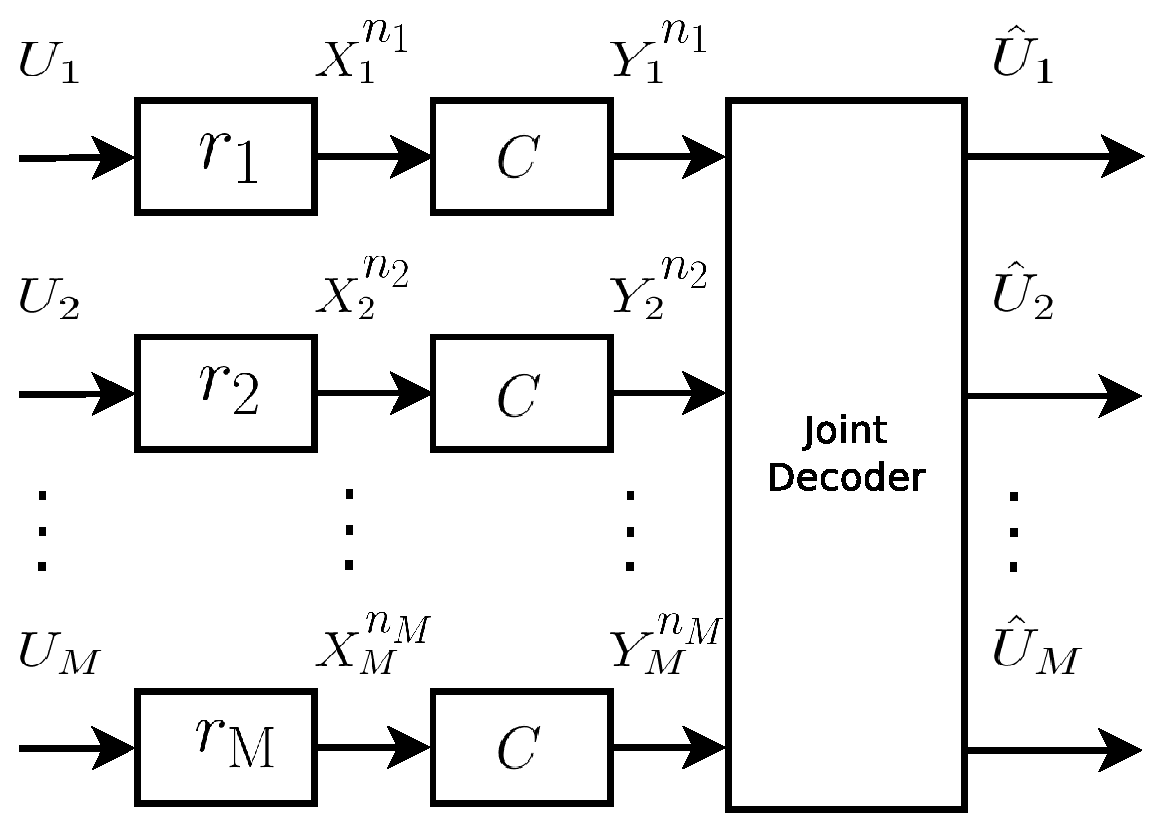
\includegraphics[width=8.0cm]{pujaico1.eps}
\caption{System Model.} \label{fig:modelo}
\end{figure}

%%%%%%%%%%%%%%%%%%%%%%%%%%%%%%%%%%%%%%%%%%%%%%%%%%%%%%%%%%%%%%%%%%%%%%%%%%%%%%
\begin{definition}
 It is assumed that the source 
$U_m$, $\forall$ $m \in$ $\{1,$ $2,$ $...,$ $M\}$, it is created 
passing a source $U_0$, with $Pr(U_0=1)=0.5$, across a BSC channel  with error 
probability $Pr(U_m \ne U_0 | U_0)=p_m$.
\end{definition}

%%%%%%%%%%%%%%%%%%%%%%%%%%%%%%%%%%%%%%%%%%%%%%%%%%%%%%%%%%%%%%%%%%%%%%%%%%%%%%
\begin{definition}
\label{def:US} 
Let $S \subseteq \{1, 2, \ldots, M\}$ be an index subset and $S^c$  your complement.
Then, $U(S)\equiv \{U_i: i \in S\}$ is the set the sources indexed by $S$, and $U(S^c)$ is the set
of sources indexed by $S^c$. 


\end{definition}
%%%%%%%%%%%%%%%%%%%%%%%%%%%%%%%%%%%%%%%%%%%%%%%%%%%%%%%%%%%%%%%%%%%%%%%%%%%%%%

\begin{lemma}
It is well known \cite{fernando} that for transmit information without
error across channels with capacity $C$, it is necessary fulfill the next
relation between the codification rate $r_m$ and the channel capacity $C$,
\begin{equation}\label{eq:gamma5_1}
H(U(S)|U(S^c)) -\sum_{i \in S}{ \frac{C}{r_i}}  \leq  0.
\end{equation}
%This article works over this issue and proposes new methods of solution. 
\end{lemma}


%%%%%%%%%%%%%%%%%%%%%%%%%%%%%%%%%%%%%%%%%%%%%%%%%%%%%%%%%%%%%%%%%%%%%%%%%%%%%%
\begin{definition}
 \label{def:omega}
Let $\Omega_m$, $\forall m \in \{1,$ $2,$ $...,$ $M\}$, be a set of the $m$ first correlated 
sources, so that 
\begin{equation}
\label{eq:omega}
 \Omega_m \equiv \{U_i: i \in \mathbf{Z^+}, 1 \leq i \leq m\};
\end{equation}
with the especial case where $\Omega_0$ equal to null, so that $H(\Omega_0)=0$.
\end{definition}

%%%%%%%%%%%%%%%%%%%%%%%%%%%%%%%%%%%%%%%%%%%%%%%%%%%%%%%%%%%%%%%%%%%%%%%%%%%%%%
\begin{definition}
Let $S_m$ be anything set of $m$ sources 
in $\Omega_M$, with the especial case of $S_0$ equal to null, so that $H(S_0)=0$. 
Also it is defined $\tilde{S}_m$ with $M-m$ sources, as the complement of 
$S_m$, so that $S_m \cup \tilde{S}_m = \Omega_M$.
\end{definition}

%%%%%%%%%%%%%%%%%%%%%%%%%%%%%%%%%%%%%%%%%%%%%%%%%%%%%%%%%%%%%%%%%%%%%%%%%%%%%%
\begin{definition}
 \label{def:hb}
The binary entropy is defined as $h_b(\rho)$, so that
\begin{equation}
\label{eq:hb1}
h_b(\rho)=- \rho ~ log_2(\rho) - (1-\rho) ~ log_2(1-\rho).
\end{equation}
If the probability $p_m$ was evaluated, then is defined
\begin{equation}
\label{eq:hi}
h_m \equiv h_b(p_m).
\end{equation}
\end{definition}

 
%%%%%%%%%%%%%%%%%%%%%%%%%%%%%%%%%%%%%%%%%%%%%%%%%%%%%%%%%%%%%%%%%%%%%%%%%%%%%%
%%%%%%%%%%%%%%%%%%%%%%%%%%%%%%%%%%%%%%%%%%%%%%%%%%%%%%%%%%%%%%%%%%%%%%%%%%%%%%
%%%%%%%%%%%%%%%%%%%%%%%%%%%%%%%%%%%%%%%%%%%%%%%%%%%%%%%%%%%%%%%%%%%%%%%%%%%%%%
\section{Optimal Common Rate} 
\label{sec:Optimo}
As is seen in \cite{fernando} and (\ref{eq:gamma5_1}), 
the calculus of optimal codification rate for the 
case where $r_m=r$ and $C_m=C$, $\forall m \in \{1, 2, ...,M\}$, it
is obtained finding the maximum value of $r$ in the next relation, 
that it is represent by a set of inequalities,
\begin{equation}\label{eq:gamma6}
 r \leq   \frac{\sum_{i \in S}{ C}}{H(U(S)|U(S^c))}.
\end{equation}
Analyzing these inequalities is easy to see that for $M$ sources is necessary do
comparisons with $2^M-1$ inequalities (number of no-null subsets in $S$), 
so that this number of comparisons grows 
exponentially with $M$ and it is not manageable.
In the next subsection will be show how simplify and reduce the equation (\ref{eq:gamma6})
to have an expression that grow linearly  with $M$.
%%%%%%%%%%%%%%%%%%%%%%%%%%%%%%%%%%%%%%%%%%%%%%%%%%%%%%%%%%%%%%%%%%%%%%%%%%%%%%
%%%%%%%%%%%%%%%%%%%%%%%%%%%%%%%%%%%%%%%%%%%%%%%%%%%%%%%%%%%%%%%%%%%%%%%%%%%%%%
%%%%%%%%%%%%%%%%%%%%%%%%%%%%%%%%%%%%%%%%%%%%%%%%%%%%%%%%%%%%%%%%%%%%%%%%%%%%%%
\subsection{Optimizing the Calculus of Optimal Common Rate} 
\label{sec:Optimizingl}

For to simplify the equation (\ref{eq:gamma6}) is necessary 
to choose each index $m$ of $U_m$, 
in ascending entropy of $h_b(p_{m})\equiv H(U_m|U_0)$, so that $h_b(p_{i}) \leq h_b(p_{i+1})$, 
$\forall i$ $\in \{1,$ $2,$ $...,$ $M-1\}$. The Table \ref{tab:1} show this relation.
\begin{table}[!hbt]
\caption{Correlated sources in ascending entropy $h_b(p_m)$}
\begin{center}
\begin{tabular}{|l |l | l | l | l |l |}
\hline
   ~       & $U_1$      & $U_2$      & $U_3$      & \dots & $U_{M}$ \\
\hline
\hline
$p_m$      & $p_1$      & $p_2$      & $p_3$      & \dots & $p_{M}$ \\
\hline
$h_b(p_m)$ & $h_1$      & $h_2$      & $h_3$      & \dots & $h_{M}$ \\
\hline
\end{tabular}
\end{center}
\label{tab:1}
\end{table}

The equation (\ref{eq:gamma6}) can be rewrite then as
\begin{equation}\label{eq:gamma_1}
 r \leq   \frac{ m C}{H(S_m|\tilde{S}_m)}.
\end{equation}
Each value $m$, $\forall m \in \{1, 2, ..., M\}$, in (\ref{eq:gamma_1}) 
represent a group of $\binom{M}{m}$ 
inequalities. As in the calculus of $r$ is indifferent the order in that the  
subsets $S_m$ are compared, the equation (\ref{eq:gamma_1}) can be 
rewrite as
\begin{equation}\label{eq:gamma_11}
 r \leq   \frac{ m C}{H(\Omega_M)-H(S_{M-m})}.
\end{equation}


Using the Lemma \ref{lemma:minimo2} of Section \ref{sec:Appendix},
we know that of all the values of $H(S_{M-m})$ in (\ref{eq:gamma_11}), we found the minimum
value to $H(\Omega_{M-m})$, so that we rewrite the equation (\ref{eq:gamma_11}) as (\ref{eq:gamma_2}),
\begin{equation}\label{eq:gamma_2}
 r \leq   \frac{ m C}{H(\Omega_{M}) - H(\Omega_{M-m})}.
\end{equation}
Thus, we just need $M$ inequalities for calculate the optimal common 
rate of $M$ sources. This imply that is necessary the calculus of 
$H(\Omega_m)$, $\forall m \in \{1, 2, ..., M\}$, such that now;
\textcolor{red}{excluding the work of calculates $H(\Omega_m)$}; the complexity is linear.
%%%%%%%%%%%%%%%%%%%%%%%%%%%%%%%%%%%%%%%%%%%%%%%%%%%%%%%%%%%%%%%%%%%%%%%%%%%%%%
%%%%%%%%%%%%%%%%%%%%%%%%%%%%%%%%%%%%%%%%%%%%%%%%%%%%%%%%%%%%%%%%%%%%%%%%%%%%%%
%%%%%%%%%%%%%%%%%%%%%%%%%%%%%%%%%%%%%%%%%%%%%%%%%%%%%%%%%%%%%%%%%%%%%%%%%%%%%%
%%%%%%%%%%%%%%%%%%%%%%%%%%%%%%%%%%%%%%%%%%%%%%%%%%%%%%%%%%%%%%%%%%%%%%%%%%%%%%
%%%%%%%%%%%%%%%%%%%%%%%%%%%%%%%%%%%%%%%%%%%%%%%%%%%%%%%%%%%%%%%%%%%%%%%%%%%%%%
%%%%%%%%%%%%%%%%%%%%%%%%%%%%%%%%%%%%%%%%%%%%%%%%%%%%%%%%%%%%%%%%%%%%%%%%%%%%%%

\section{Optimal Sum Rate} \label{sec:sumrate}
\begin{remark}
\textcolor{red}{Na quinta linha do artigo \cite{fernando} diz: ``we chose to formulate it as the following equivalent problem;'' 
e tem que dizer ``we chose formulate instead it the following similar problem;'' debido a que a solucao $\mathbf{n^*}$
que minimiza $\sum_{i}n^*_i=S$ contem a solucao $\mathbf{n^a}$
que maximiza $\sum_{i}\frac{1}{n^a_i}=T$ , mas nao todos os $\mathbf{n^*}$ encontrados
maximizam $\mathbf{n^a}$. Exemplo:$\mathbf{n^*}=(3,3) \rightarrow S=6$ e $\mathbf{n^*}=(2,4) \rightarrow S=6$; agora
los valores inversos serian $\mathbf{1/n^*}=(1/3,1/3) \rightarrow T=\frac{3}{2}=0.6667$ 
e $\mathbf{1/n^*}=(1/2,1/4) \rightarrow T=\frac{3}{4}=0.75$, respectivamente.}
\end{remark}

\begin{remark}
\textcolor{red}{En el ejemplo 4 depois da equacao (30) diz`` represents the set of solutions that minimize the sum''
e deve dizer ``contents the set of solutions that minimize the sum''.}

\textcolor{red}{
Pois, falta a restrição de que $n^*_i\geq k$ and consequently $1/k\geq 1/n^*_i$
e outras restricoes do slepian wolf theorem}
\end{remark}

In \cite{fernando} can be seen that, the problem of maximize $\sum_{m=1}^{M}{ r_m}$ 
is equivalent to minimize the sum $N=\sum_{m=1}^{M}{ n_m}$. 
Follow  (\ref{eq:gamma5_1}) and \cite{fernando}, we know that for minimize $N$ 
we are restricted to  that the 
lengths $n_m$ (of rates $r_m=k/n_m$ , $\forall m \in \{1, 2, ..., M\}$), fulfill the next inequalities,
\begin{equation}\label{eq:sumrate1}
  \sum_{i \in S}{n_i}\geq \frac{k}{C} H(U(S)|U(S^c)).
\end{equation}
The M-tuples that fulfill the last equation are represent for $\mathbf{n}=(n_1,n_2, ..., n_M)$.
Thus, is necessary
to get
%\begin{equation}\label{eq:sumrate0a}
%N=\sum_{m=1}^{M}{ n_m},
%\end{equation}
\begin{equation}\label{eq:sumrate0}
\mathbf{n^*}=\arg{ \min \limits_{\{n_m\}}{N} },
\end{equation}
restrict to (\ref{eq:sumrate1}),
where $\mathbf{n^*}=(n^*_1, n^*_2, ..., n^*_M)$ represents the M-tuples of 
$\mathbf{n}$ that minimize $N$. 
In \cite{fernando} can be seen that for to get these values 
is necessary to solve a matrix inequation with $M$ columns a $2^{M}-1$ rows.
\subsection{Calculus of Optimal Sum Rate } \label{subsec:sumratemethod}
If we see the equation (\ref{eq:sumrate1}), it is easy to perceive that the bounded
region of this equation is proportional to the bounded region of Slepian-Wolf
theorem  \cite{slepian,cover}. Thus, the possibles values of M-tuple 
$\mathbf{n}$ are equals to $\mathbf{n} = \frac{k}{C} \mathbf{R}$,
where the M-tuple $\mathbf{R}=(R_1,R_2, ..., R_M)$ represent the possibles informations rates
in the bounded region of Slepian-Wolf Theorem. Known
this, (\ref{eq:sumrate0}) can be rewrite as (\ref{eq:sumrate01}),
\begin{equation}\label{eq:sumrate01}
\mathbf{n^*}= \frac{k}{C} \arg{\min \limits_{\{R_m\}}{\sum_{m=1}^{M}{ R_m} }},
\end{equation}
so that 
\begin{equation}\label{eq:sumrate01a}
H(U(S)|U(S^c)) \leq \sum_{i\in S}{ R_i}.
\end{equation}

By other side, in \cite{cornersuperfluo,cornerqualquer,cornerpesos} 
we can see that, the corner points $\mathbf{R^*}=(R^*_1,R^*_2, ..., R^*_M)$ 
that pertain to $\mathbf{R}$, 
and also delimit  with segments a hyperplane portion $\ell_0$  inside
$\ell :\sum_{m=1}^{M}{ R_m}=H(U_1 U_2 ... U_M)$,
they represent solutions that
minimize the sum $\sum_{m=1}^{M}{ R_m }$ conditioned to (\ref{eq:sumrate01a}), 
being that these solutions are not uniques 
and any point inside $\ell_0$ also minimize the sum. 

Consequently, the corner points $\mathbf{R^*}$
describe the outline of solution region $\ell_0$,
these M-tuples can be obtained by expanding $H(U_1 U_2 ... U_M)$,
by successive applications of the chain rule in any order, and assigning to each 
rate $R^*_m$ the term in the expansion that correspond to the 
analyzed source in the entropy function \cite{cornersuperfluo}. By example,
in the bi-dimensional case with a $H(U_2 U_1)$, the corner points $(R^*_1,R^*_2)$ 
of $\ell_0$ are in $(H(U_1|U_2),H(U_2))$ 
and $(H(U_1), H(U_2|U_1))$; by other side, to the multidimensional case one corner point can be
\begin{equation}\label{eq:R}
\begin{matrix}
R^*_i&=&H(U_i|U_{i-1} U_{i-2} ... U_{1})\\
~    &=&H(\Omega_i)-H(\Omega_{i-1}),
\end{matrix}
\end{equation}
for $i \in \{1, 2, ..., M-1\}$ with $R^*_1=H(U_1)$.

By (\ref{eq:R}), we know that the equation (\ref{eq:sumrate0}) has one solution
in
\small
\begin{equation}\label{eq:sumratefinal}
\mathbf{n^*}=\frac{k}{C} \left(
\begin{matrix}
 H(U_1)\\
 H(\Omega_2)-H(U_{1})\\
 \vdots \\
 H(\Omega_i)-H(\Omega_{i-1})\\
 \vdots \\   
 H(\Omega_M)-H(\Omega_{M-1})
\end{matrix}
\right)^T.
\end{equation}
\normalsize
Thus, for calculate the optimal sum rate of $M$ sources imply that is necessary 
the calculus of $H(\Omega_m)$, $\forall m \in \{1, 2, ..., M\}$.
%%%%%%%%%%%%%%%%%%%%%%%%%%%%%%%%%%%%%%%%%%%%%%%%%%%%%%%%%%%%%%%%%%%%%%%%%%%%%%
%%%%%%%%%%%%%%%%%%%%%%%%%%%%%%%%%%%%%%%%%%%%%%%%%%%%%%%%%%%%%%%%%%%%%%%%%%%%%%
%%%%%%%%%%%%%%%%%%%%%%%%%%%%%%%%%%%%%%%%%%%%%%%%%%%%%%%%%%%%%%%%%%%%%%%%%%%%%%
%%%%%%%%%%%%%%%%%%%%%%%%%%%%%%%%%%%%%%%%%%%%%%%%%%%%%%%%%%%%%%%%%%%%%%%%%%%%%%
\section{Final Remarks and Conclusions} 
\label{sec:Conclusions}
In this letter, we considered joint source-channel coding of correlated
sources transmitted over orthogonal channels with the same channel capacity, 
and were solved two optimization problems focusing on the computation low complexity  
of optimal rates calculus. 
It is therefore expected that the optimal rates derived in this letter can
serve as guidance to practical coding schemes.

But remain open the search of a method of 
calculus of the joint entropy $H(\Omega_m)$. This entropy yet need much calculus
time. Analyzing this problem is recommended for futures works that the problem
be addressed as an approximate calculation.

%%%%%%%%%%%%%%%%%%%%%%%%%%%%%%%%%%%%%%%%%%%%%%%%%%%%%%%%%%%%%%%%%%%%%%%%%%%%%%
%%%%%%%%%%%%%%%%%%%%%%%%%%%%%%%%%%%%%%%%%%%%%%%%%%%%%%%%%%%%%%%%%%%%%%%%%%%%%%
%%%%%%%%%%%%%%%%%%%%%%%%%%%%%%%%%%%%%%%%%%%%%%%%%%%%%%%%%%%%%%%%%%%%%%%%%%%%%%
\section*{Acknowledgment}

H(Omega) no lo calcules !!!simulalo!!!


%%%%%%%%%%%%%%%%%%%%%%%%%%%%%%%%%%%%%%%%%%%%%%%%%%%%%%%%%%%%%%%%%%%%%%%%%%%%%%
%\appendix
\section{Appendix} \label{sec:Appendix}

%%%%%%%%%%%%%%%%%%%%%%%%%%%%%%%%%%%%%%%%%%%%%%%%%%%%%%%%%%%%%%%%%%%%%%%%%%%%%%
\begin{lemma}
 \label{lemm:PrA}
Known a set of $m$ correlated  sources  $\Omega_m$. Then, is true that
\begin{equation}\label{eq:PA}
Pr(\Omega_m=\mathbf{a})=\frac{ \Psi(\mathbf{a}) + \Psi(\mathbf{\bar{a}}) }{2},
\end{equation}
\begin{equation}\label{eq:PAequiv}
\Psi(\mathbf{a}) \equiv \prod \limits_{i=1}^{m}{Pr(U_i=a_i|U_0=0)}.
\end{equation}
being $\mathbf{a}=\{a_1, a_2, ..., a_m\}$ and $\mathbf{\bar{a}}$ two 
binary vectors, both with $m$ elements, where $\mathbf{\bar{a}}\oplus \mathbf{a}=\mathbf{0}$. 
\end{lemma}
\begin{proof}
 \label{proof:PrA} 
\begin{equation}\label{eq:PA1}
\begin{matrix}
Pr(\Omega_m=\mathbf{a})&=&Pr(\Omega_m=\mathbf{a}|U_0=0)Pr(U_0=0)\\
~                 &+&Pr(\Omega_m=\mathbf{a}|U_0=1)Pr(U_0=1), 
\end{matrix}
\end{equation}
%\begin{equation}\label{eq:PA2}
%\begin{matrix}
%Pr(\Omega_m=\mathbf{a})&=&(1/2)Pr(\Omega_m=\mathbf{a}|U_0=0)\\
%~                      &+&(1/2)Pr(\Omega_m=\mathbf{a}|U_0=1), 
%\end{matrix}
%\end{equation}
when $U_0$ is known the probabilities of sources in $\Omega_m$ are independents,
\begin{equation}\label{eq:PA3}
\begin{matrix}
Pr(\Omega_m=\mathbf{a})&=&(1/2)\prod \limits_{U_i\in \Omega_m}{Pr(U_i=a_i|U_0=0)}\\
~                      &+&(1/2)\prod \limits_{U_i\in \Omega_m}{Pr(U_i=a_i|U_0=1)}, 
\end{matrix}
\end{equation}
\end{proof}


%%%%%%%%%%%%%%%%%%%%%%%%%%%%%%%%%%%%%%%%%%%%%%%%%%%%%%%%%%%%%%%%%%%%%%%%%%%%%%
\begin{lemma}
 \label{lemm:hpi} 
The value of entropy function $H(\Omega_m)$ is the same for a set of sources
$U_i$ with $Pr(U_i\neq U_0|U_0)$ equal to $p_i$ or $1-p_i$
\end{lemma}
\begin{proof}
 \label{proof:hpi} 
Without loss of generality, we assume that need demonstrate $H(U_i\Omega_{m})$
is the same for $Pr(U_i\neq U_0|U_0)$ equal to $p_i$ or $1-p_i$.
\begin{equation}\label{eq:hpi1}
\begin{matrix}
H(U_i\Omega_{m})\\
=\sum \limits_{U_i,\Omega_{m}} Pr(U_i\Omega_{m}) log_2(Pr(U_i\Omega_{m})) ~~~~~~~~~~~~~~~~~~~~\\
=\sum \limits_{\mathbf{a}} Pr(U_i=1,\Omega_{m}=\mathbf{a}) log_2(Pr(U_i=1,\Omega_{m}=\mathbf{a}))\\
+\sum \limits_{\mathbf{a}} Pr(U_i=0,\Omega_{m}=\mathbf{a}) log_2(Pr(U_i=0,\Omega_{m}=\mathbf{a}))
\end{matrix}
\end{equation}
Using the Lemma \ref{lemm:PrA} we know that for the case of $Pr(U_i\neq U_0|U_0)=p_i$ 
\begin{equation}\label{eq:hpi2}
Pr(U_i=1,\Omega_m=\mathbf{a})=\frac{ p_i\Psi(\mathbf{a}) + (1-p_i)\Psi(\mathbf{\bar{a}}) }{2},
\end{equation}
\begin{equation}\label{eq:hpi3}
Pr(U_i=0,\Omega_m=\mathbf{a})=\frac{ (1-p_i)\Psi(\mathbf{a}) + p_i\Psi(\mathbf{\bar{a}}) }{2},
\end{equation}
and for the case of $Pr(U_i\neq U_0|U_0)=1-p_i$
\begin{equation}\label{eq:hpi4}
Pr(U_i=1,\Omega_m=\mathbf{a})=\frac{ (1-p_i)\Psi(\mathbf{a}) + p_i\Psi(\mathbf{\bar{a}}) }{2},
\end{equation}
\begin{equation}\label{eq:hpi5}
Pr(U_i=0,\Omega_m=\mathbf{a})=\frac{ p_i\Psi(\mathbf{a}) + (1-p_i)\Psi(\mathbf{\bar{a}}) }{2}.
\end{equation}
Using this results is easy see that for both case  we obtain the same value of 
$H(U_i\Omega_{m})$.
\end{proof}
%%%%%%%%%%%%%%%%%%%%%%%%%%%%%%%%%%%%%%%%%%%%%%%%%%%%%%%%%%%%%%%%%%%%%%%%%%%%%%
\begin{corollary}
 \label{coro:hpi} 
Follow the Lemma \ref{lemm:hpi}, for calculate the joint entropy $H(\Omega_m)$ 
we can assume that all probabilities $p_i \leq 1/2$. Thus, exist a bijective 
function that link the probability $p_i$ an the binary entropy $h_i$. Therefore
the joint entropy $H(\Omega_m)$ is a function that depend of $\mathbf{h}=\{h_1, h_2, ..., h_m\}$.
\end{corollary}




%%%%%%%%%%%%%%%%%%%%%%%%%%%%%%%%%%%%%%%%%%%%%%%%%%%%%%%%%%%%%%%%%%%%%%%%%%%%%%
\begin{lemma}
 \label{lemm:dH}
Known a set of $m$ correlated  sources  $\Omega_m$. Then, is true that
the value of entropy $H(\Omega_m)$ grow in relation growing of $h_b(p_i)$, 
$\forall i$ $\in \{1,$ $2,$ $...,$ $m\}$, so that
\begin{equation}\label{eq:dH1}
 \frac{\partial H(\Omega_m)}{\partial h_i} \geq 0
\end{equation}
\end{lemma}
\begin{proof}
 \label{proof:dH} 
For the Corollary \ref{coro:hpi} we know that $H(\Omega_m)$ depend of $h_i$
and this depend of $p_i$. Without loss of generality, 
we assume that need demonstrate
$({\partial H(U_j\Omega_{m})}/{\partial p_j}) ({\partial p_j}/{\partial h_j}) \geq 0$,
being that $U_j \notin \Omega_{m}$. Thus,
\small
\begin{equation}\label{eq:dH2}
 \frac{\partial H(U_j\Omega_{m})}{\partial h_j} =\frac{-\partial \sum \limits_{U_j,\Omega_{m}} Pr(U_j\Omega_{m}) log_2(Pr(U_j\Omega_{m}))}{\partial p_j}\frac{\partial p_j}{\partial h_j} 
\end{equation}
\normalsize
%\small
\begin{equation}\label{eq:dH21}
\begin{matrix}
\frac{\partial H(U_j\Omega_{m})}{\partial h_j} =\\
-\frac{\partial \sum \limits_{\mathbf{a}} Pr(U_j=1,\Omega_{m}=\mathbf{a}) log_2(Pr(U_j=1,\Omega_{m}=\mathbf{a}))}{\partial p_j}\frac{\partial p_j}{\partial h_j}  \\
-\frac{\partial \sum \limits_{\mathbf{a}} Pr(U_j=0,\Omega_{m}=\mathbf{a}) log_2(Pr(U_j=0,\Omega_{m}=\mathbf{a}))}{\partial p_j}\frac{\partial p_j}{\partial h_j}
\end{matrix}
\end{equation}
%\normalsize
and using the Lemma \ref{lemm:PrA} we obtain
\begin{equation}\label{eq:dH3}
 Pr(U_j=1,\Omega_{m}=\mathbf{a})=\frac{ p_j\Psi(\mathbf{a}) + (1-p_j)\Psi(\mathbf{\bar{a}}) }{2},
\end{equation}
\begin{equation}\label{eq:dH4}
 Pr(U_j=0,\Omega_{m}=\mathbf{a})=\frac{ (1-p_j)\Psi(\mathbf{a}) + p_j\Psi(\mathbf{\bar{a}}) }{2},
\end{equation}
\begin{equation}\label{eq:dH6}
 \frac{\partial Pr(U_j=1,\Omega_{m}=\mathbf{a})}{\partial p_j}=\frac{ \Psi(\mathbf{a}) -\Psi(\mathbf{\bar{a}}) }{2},
\end{equation}
\begin{equation}\label{eq:dH7}
 \frac{\partial Pr(U_j=0,\Omega_{m}=\mathbf{a})}{\partial p_j}=-\frac{ \Psi(\mathbf{a}) -\Psi(\mathbf{\bar{a}}) }{2},
\end{equation}
\begin{equation}\label{eq:dH5}
 \frac{\partial h_j}{\partial p_j}=log_2 \left( \frac{1-p_j}{p_j}\right),
\end{equation}
using (\ref{eq:dH3}), (\ref{eq:dH4}), (\ref{eq:dH6}), (\ref{eq:dH7}) and (\ref{eq:dH5}) in (\ref{eq:dH21})
\begin{equation}\label{eq:dH22}
\frac{\partial H(U_j\Omega_{m})}{\partial h_j} = \sum \limits_{\mathbf{a}} f(p_j,\mathbf{a})
\end{equation}
\begin{equation}\label{eq:dH23}
f(p_j,\mathbf{a}) = \frac{ \Psi(\mathbf{a}) -\Psi(\mathbf{\bar{a}}) }{2~log_2 \left( \frac{1-p_j}{p_j}\right)} log_2\left( \frac{ (1-p_j)\Psi(\mathbf{a}) + p_j\Psi(\mathbf{\bar{a}}) }{ p_j\Psi(\mathbf{a}) + (1-p_j)\Psi(\mathbf{\bar{a}}) }\right)
\end{equation}
if $p_j=1/2$, then
\begin{equation}\label{eq:dH24}
f(1/2,\mathbf{a}) = \frac{1}{2}\frac{ (\Psi(\mathbf{a}) -\Psi(\mathbf{\bar{a}}))^2 }{\Psi(\mathbf{a}) + \Psi(\mathbf{\bar{a}})} \geq 0.
\end{equation}
Analyzing the equation (\ref{eq:dH23}) for $p_j<1/2$, $p_j>1/2$, 
$\Psi(\mathbf{a}) \leq \Psi(\mathbf{\bar{a}})$ and $\Psi(\mathbf{a}) > \Psi(\mathbf{\bar{a}})$,
can be seen that $f(p_j,\mathbf{a})$ is ever positive, thus the Lemma \ref{lemm:dH} 
is proved.
\end{proof}
%%%%%%%%%%%%%%%%%%%%%%%%%%%%%%%%%%%%%%%%%%%%%%%%%%%%%%%%%%%%%%%%%%%%%%%%%%%%%%
\begin{corollary}
 \label{corol:dH}  We know that  $H(\Omega_m)$
is in function of $\mathbf{h}=\{h_1, h_2, ..., h_m\}$, thus 
$H(\Omega_m) = \phi(\mathbf{h})$, where $\phi(.)$ is a $m$-dimensional function.
Follow the Lemma \ref{lemm:dH} we know that
\begin{equation}\label{eq:coro1}
\phi(\mathbf{h}) \leq \phi(\mathbf{h} +  \mathbf{\triangle h}) 
\end{equation}
when the elements of $\mathbf{\triangle h}$ are higher or equal to zero.
\end{corollary}
%%%%%%%%%%%%%%%%%%%%%%%%%%%%%%%%%%%%%%%%%%%%%%%%%%%%%%%%%%%%%%%%%%%%%%%%%%%%%%
\begin{lemma}
\label{lemma:minimo2}
Known $M$ correlated sources with indexes chosen in ascending entropy 
$h_b(p_m)$, $\forall m$ $\in \{1,$ $2,$ $...,$ $M\}$, as in the Table \ref{tab:1}.
If we select two set of $m$ sources, $\Omega_m$ and $S_m$,
then
\begin{equation}
H(\Omega_m) \leq H(S_m),
\end{equation}
\end{lemma}
\begin{proof}
\label{proof:minimo2}
The joint entropy $H(S_m)$ is in function of a set probabilities
$p_i=P(U_i\neq U_0|U_0)$, $\forall i: U_i \in S_m$. For the symmetry 
of entropy function, the order of $p_i$ is irrelevant for the calculus of 
$H(S_m)$. We define $\mathbf{\tilde{h}}$ as a set of binary entropies,
in ascending order, of all probabilities $p_i$ linked to $S_m$.
Knowing this, we can say that the entropies $H(\Omega_m)$ and $H(S_m)$ are in function of 
two sets of $m$ entropies 
$\mathbf{h}=\{h_{1},$ $h_{2},$ $...,$ $h_{m}\}$ and
$\mathbf{\tilde{h}}=\{\tilde{h}_{1},$ $\tilde{h}_{2},$ $...,$ $\tilde{h}_{m}\}$ respectively, being that 
both are write in ascending entropy. By definition of problem $\mathbf{h}$ have
a set of entropies with lower values, the other hand $\mathbf{\tilde{h}}$ is a 
set of $m$ anybody entropies $h_i$ in the Table \ref{tab:1}. Given that
element to element $\mathbf{\tilde{h}}$ ever will be major than $\mathbf{h}$ and
using the Corollary \ref{corol:dH} we know that $\phi(\mathbf{h}) \leq \phi(\mathbf{\tilde{h}})$
and the Lemma \ref{lemma:minimo2} is proved.
\end{proof}

%%%%%%%%%%%%%%%%%%%%%%%%%%%%%%%%%%%%%%%%%%%%%%%%%%%%%%%%%%%%%%%%%%%%%%%%%%%%%%
%%%%%%%%%%%%%%%%%%%%%%%%%%%%%%%%%%%%%%%%%%%%%%%%%%%%%%%%%%%%%%%%%%%%%%%%%%%%%%
%%%%%%%%%%%%%%%%%%%%%%%%%%%%%%%%%%%%%%%%%%%%%%%%%%%%%%%%%%%%%%%%%%%%%%%%%%%%%%
\begin{thebibliography}{99}

\bibitem{fernando} Pujaico, F.; Portugheis, J.,
``Optimal Rate for Joint Source-Channel Coding of Correlated Sources Over 
Orthogonal Channels,'' Communications Letters, 2014.

\bibitem{slepian} Slepian, D.; Wolf, J.K., 
``Noiseless coding of correlated information sources,'' 
Information Theory, IEEE Transactions on , vol.19, no.4, pp.471,480, Jul 1973.

\bibitem{cover}
T. M. Cover, and J. Thomas, \textit{Elements of Information Theory}, Wiley-Interscience, 2006.

\bibitem{corrspatial} Oldewurtel, F.; Ansari, J.; Mahonen, P., 
``Cross-Layer Design for Distributed Source Coding in Wireless Sensor Networks,'' 
Sensor Technologies and Applications, 2008. SENSORCOMM '08. Second International 
Conference on , vol., no., pp.435,443, 25-31 Aug. 2008.

\bibitem{ceobinary1} Haghighat, J.; Behroozi, Hamid; Plant, D.V., 
``Iterative joint decoding for sensor networks with binary CEO model,'' 
Signal Processing Advances in Wireless Communications, 2008. SPAWC 2008. 
IEEE 9th Workshop on , vol., no., pp.41,45, 6-9 July 2008.

\bibitem{ceobinary2} Ferrari, G.; Martalo, M.; Abrardo, A.; Raheli, R., 
``Orthogonal multiple access and information fusion: How many observations are needed?,'' 
Information Theory and Applications Workshop (ITA), 2012 , vol., no., pp.311,320, 5-10 Feb. 2012.


\bibitem{cornersuperfluo}
Coleman, T.P.; Lee, A.H.; Medard, M.; Effros, M., ``Low-Complexity Approaches to Slepian-Wolf 
Near-Lossless Distributed Data Compression,'' 
Information Theory, IEEE Transactions on , vol.52, no.8, pp.3546,3561, Aug. 2006

\bibitem{cornerqualquer}
Schonberg, D.; Ramchandran, K.; Pradhan, S.S., 
``Distributed code constructions for the entire Slepian-Wolf rate region for arbitrarily correlated sources,'' 
Data Compression Conference, 2004. Proceedings. DCC 2004 , vol., no., pp.292,301, 23-25 March 2004.

\bibitem{cornerpesos}
Cristescu, R.; Beferull-Lozano, B.; Vetterli, M., ``On network correlated data gathering,'' 
INFOCOM 2004. Twenty-third AnnualJoint Conference of the IEEE Computer and Communications Societies, 
vol.4, no., pp.2571,2582 vol.4, 7-11 March 2004.


\end{thebibliography}

\end{document}


%%%%%%%%%%%%%%%%%%%%%%%%%%%%%%%%%%%%%%%%%%%%%%%%%%%%%%%%%%%%%%%%%%%%%%%%%%%%%%
%%%%%%%%%%%%%%%%%%%%%%%%%%%%%%%%%%%%%%%%%%%%%%%%%%%%%%%%%%%%%%%%%%%%%%%%%%%%%%
%%%%%%%%%%%%%%%%%%%%%%%%%%%%%%%%%%%%%%%%%%%%%%%%%%%%%%%%%%%%%%%%%%%%%%%%%%%%%%
%%%%%%%%%%%%%%%%%%%%%%%%%%%%%%%%%%%%%%%%%%%%%%%%%%%%%%%%%%%%%%%%%%%%%%%%%%%%%%
%%%%%%%%%%%%%%%%%%%%%%%%%%%%%%%%%%%%%%%%%%%%%%%%%%%%%%%%%%%%%%%%%%%%%%%%%%%%%%
%%%%%%%%%%%%%%%%%%%%%%%%%%%%%%%%%%%%%%%%%%%%%%%%%%%%%%%%%%%%%%%%%%%%%%%%%%%%%%
%%%%%%%%%%%%%%%%%%%%%%%%%%%%%%%%%%%%%%%%%%%%%%%%%%%%%%%%%%%%%%%%%%%%%%%%%%%%%%
%%%%%%%%%%%%%%%%%%%%%%%%%%%%%%%%%%%%%%%%%%%%%%%%%%%%%%%%%%%%%%%%%%%%%%%%%%%%%%
%%%%%%%%%%%%%%%%%%%%%%%%%%%%%%%%%%%%%%%%%%%%%%%%%%%%%%%%%%%%%%%%%%%%%%%%%%%%%%
%%%%%%%%%%%%%%%%%%%%%%%%%%%%%%%%%%%%%%%%%%%%%%%%%%%%%%%%%%%%%%%%%%%%%%%%%%%%%%
%%%%%%%%%%%%%%%%%%%%%%%%%%%%%%%%%%%%%%%%%%%%%%%%%%%%%%%%%%%%%%%%%%%%%%%%%%%%%%
%%%%%%%%%%%%%%%%%%%%%%%%%%%%%%%%%%%%%%%%%%%%%%%%%%%%%%%%%%%%%%%%%%%%%%%%%%%%%%

